\documentclass{foxelas_report}

\graphicspath{{images/}}
\usepackage{pmboxdraw}
\usepackage{float}


\title{Result Analysis and Discussion}

\author{}
\date{}

\usepackage{breakcites}


\begin{document}


\maketitle

%\thispagestyle{empty}


\section{Problem Definition}
Create a NN-based model that predicts sensor values using past data as reference. 

\section{Contents}
prediction\_with\_nn\_for\_weather\_data/\\
│\\
├── report/\\
│     ├── images/\\
│     ├── report.tex\\
│     ├── report.pdf\\
│     └── foxelas\_report.cls\\
│   \\
├── config.ini\\
├── main.py\\
├── part1.py\\
├── part2.py\\
├── case1.txt\\
├── case2.txt\\
└── wheather\_data.csv\\

Run settings can be updated in config.ini. Afterwards, run 'main.py' and see the results. \\
This code was tested with PyCharm using Python 3.9 and Tensorflow 2.8.3.


\section{Data Preprocessing}
\textbf{Data type}: Time series in .csv format\\
\textbf{Variables}: id, timestamp, value, identifier, value\_type\_id, location\_id, source\_id\\

\textbf{Preprocesssing}: \\
Scale numerical variables with MinMax Scaler.\\
Convert categorical variables into multiple binary variables using One Hot Encoding.\\
Convert string into datetime. \\

\textbf{Datetime variables}: timestamp\\
\textbf{Numeric Variables}: value
\begin{figure}[H]
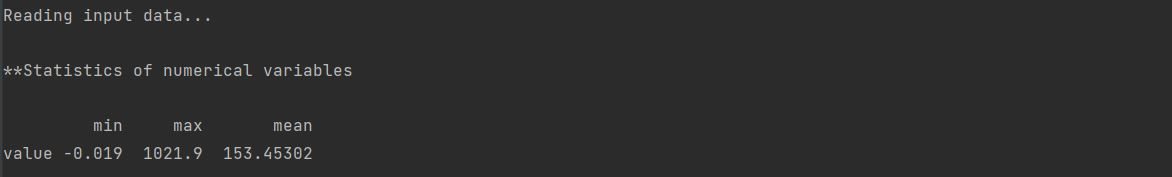
\includegraphics[width=0.9\textwidth]{img1.JPG}
\end{figure}

\textbf{Categorical Variables}: identifier
\begin{figure}[H]
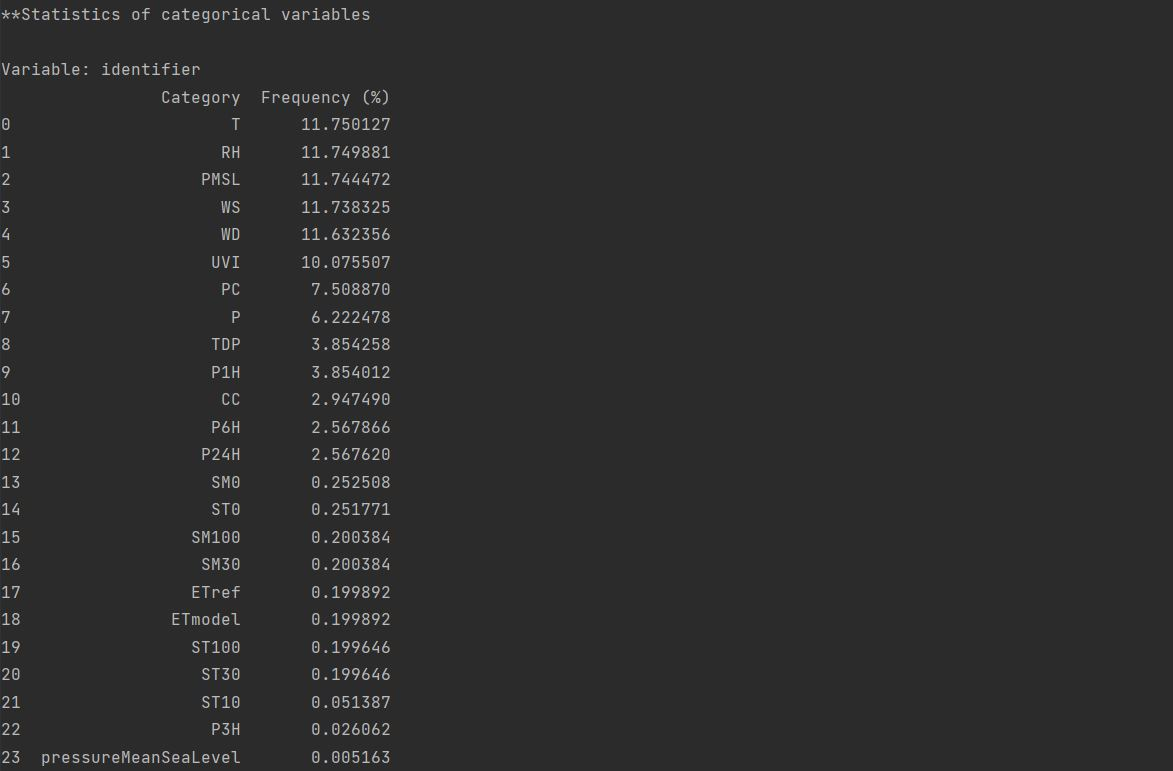
\includegraphics[width=0.9\textwidth]{img2.JPG}
\end{figure}

\textbf{Values after preprocessing}:\\

\begin{figure}[H]
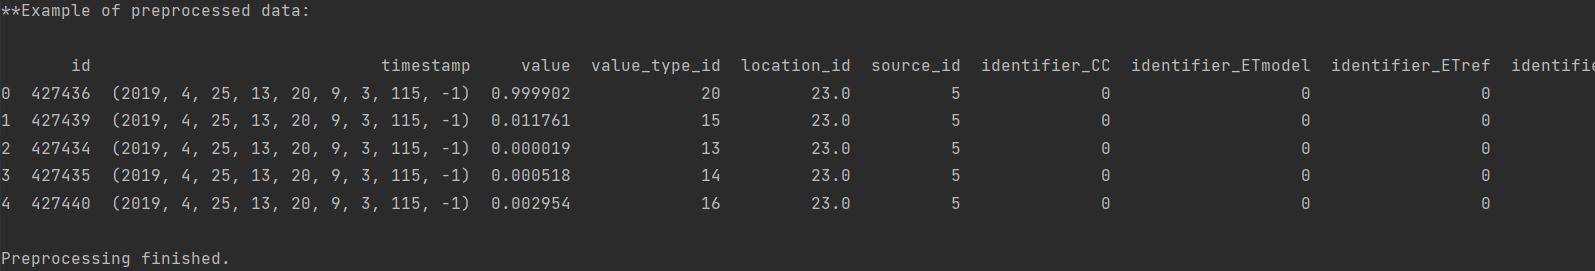
\includegraphics[width=0.9\textwidth]{img3.JPG}
\end{figure}

\textbf{Observation}: \\
For a given location\_id and value\_type\_id, all remaining variables are the same apart from columns 'timestamp' and 'value'. Therefore, the rest can be ignored in this case. 

\pagebreak
\textbf{Visualization}:\\

\begin{figure}[H]
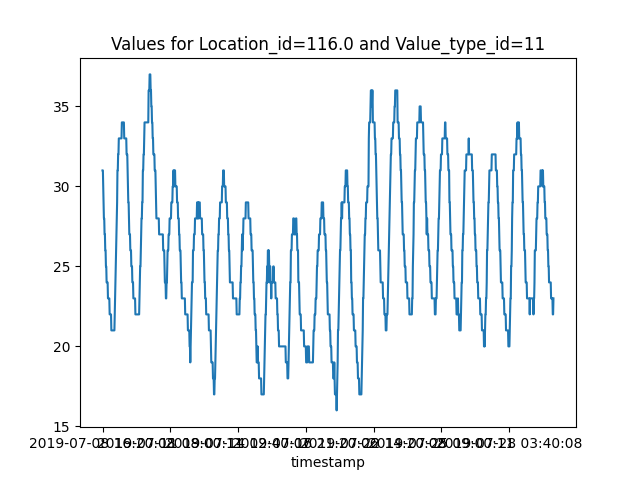
\includegraphics[width=0.6\textwidth]{vis_data_11_116.0.png}
\end{figure}

\begin{figure}[H]
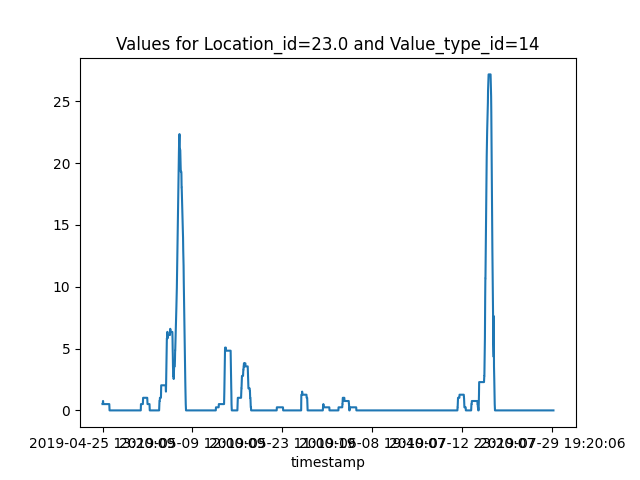
\includegraphics[width=0.6\textwidth]{vis_data_14_23.0.png}
\end{figure}

\begin{figure}[H]
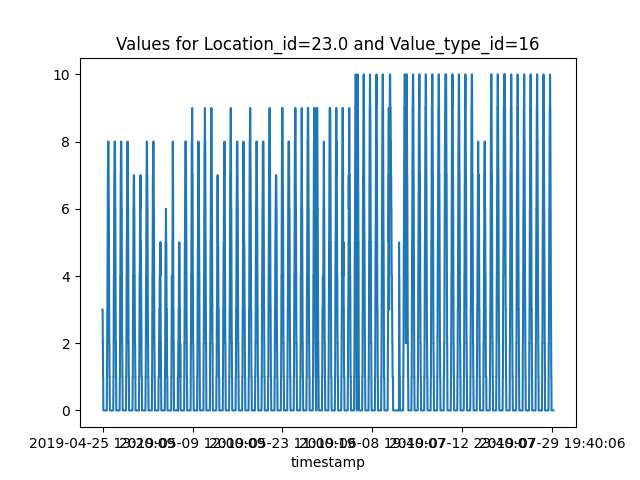
\includegraphics[width=0.6\textwidth]{vis_data_16_23.0.png}
\end{figure}

\section{Prediction Model}
A value should be predicted from previous values. A simple NN model is used (alternatively, LSTM and GRU networks are recommended).  A look-back window is applied sequentially, in order to use the n-th previous values to predict the (n+1)-th. The dataset is split in train and test subsets, in order to evaluate performance. The model is fitted on the train data, and evaluated on both train and test sets.\\

\subsection{Experiment 1}

Settings:\\
location\_id = 116.0\\
value\_type\_id = 11\\
activation = relu\\
layers\_number = 3\\
neurons\_number = [32, 16, 8, 4]\\
loss = mean\_squared\_error\\
optimizer\_name = Adam\\
epochs = 200\\
batch\_size = 32\\
window\_size = 20
split\_percentage = 0.2



The evolution of the loss function across 200 epochs for the train and test sets. Training loss is expected lower than test loss, due to fitting of the model on the train data. 

\begin{figure}[H]
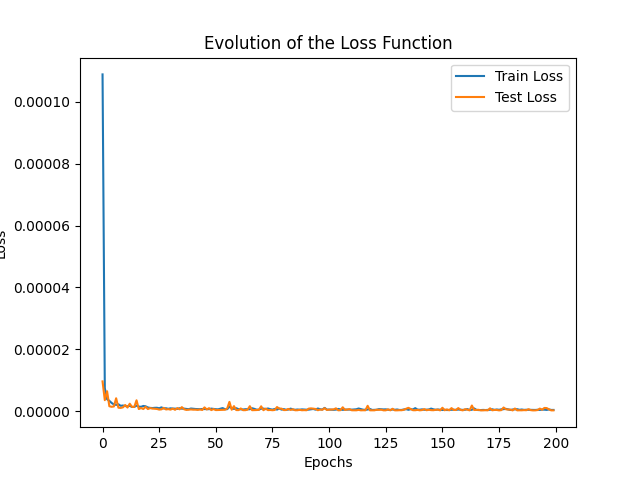
\includegraphics[width=0.6\textwidth]{case1_model_loss.png}
\end{figure}

Expected and predicted values based on the past 20 values (20 point window). The model misses the steps in the data and incorrectly predicts smoother evolution of the signal. 

\begin{figure}[H]
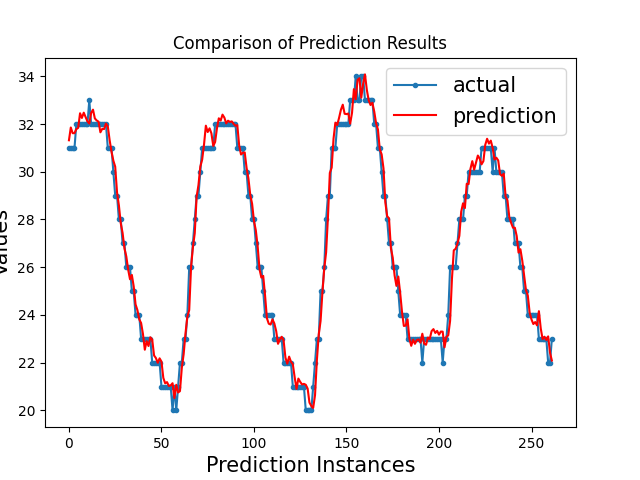
\includegraphics[width=0.6\textwidth]{case1_predictions.png}
\end{figure}

Data columns (past 20 values) are judged in terms of their contribution in the prediction using SHAP values. Values closer to the value to be predicted (last values in the window) are more influential. 

\begin{figure}[H]
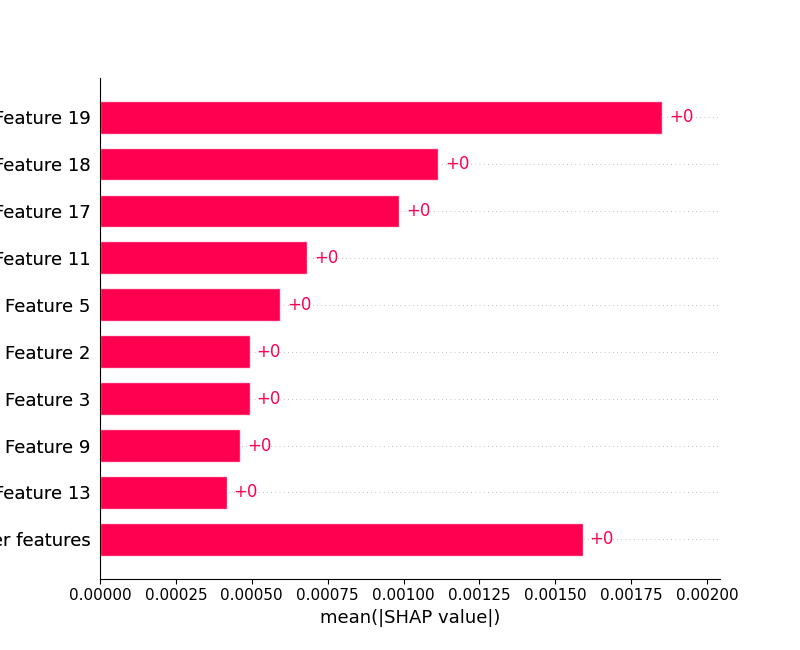
\includegraphics[width=0.6\textwidth]{case1_shap_values.png}
\end{figure}



\subsection{Experiment 2}

Settings:\\
location\_id = 116.0\\
value\_type\_id = 11\\
activation = sigmoid\\
layers\_number = 4\\
neurons\_number = [32, 16, 8, 4, 4]\\
loss = mean\_squared\_error\\
optimizer\_name = SGD\\
epochs = 200\\
batch\_size = 32\\
window\_size = 20\\
split\_percentage = 0.2\\



The evolution of the loss function across 200 epochs for the train and test sets. The shape of the curve at the knee shows that the model is not properly trained.

\begin{figure}[H]
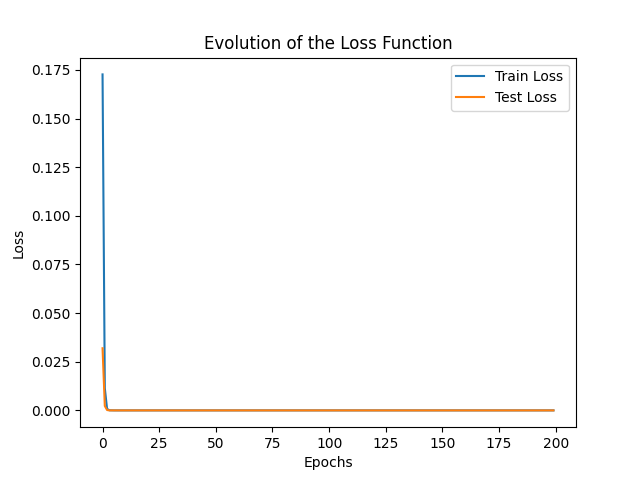
\includegraphics[width=0.6\textwidth]{case2_model_loss.png}
\end{figure}

Expected and predicted values based on the past 20 values (20 point window). The model missed the prediction completely.

\begin{figure}[H]
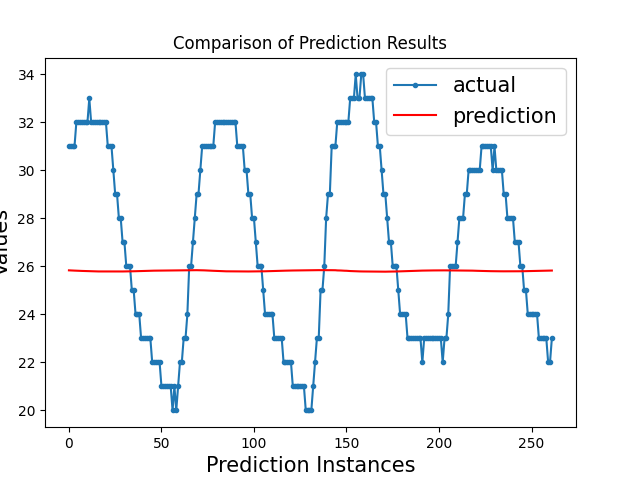
\includegraphics[width=0.6\textwidth]{case2_predictions.png}
\end{figure}

Data columns (past 20 values) are judged in terms of their contribution in the prediction using SHAP values. All of the values contribute equally to the (failed) prediction. 

\begin{figure}[H]
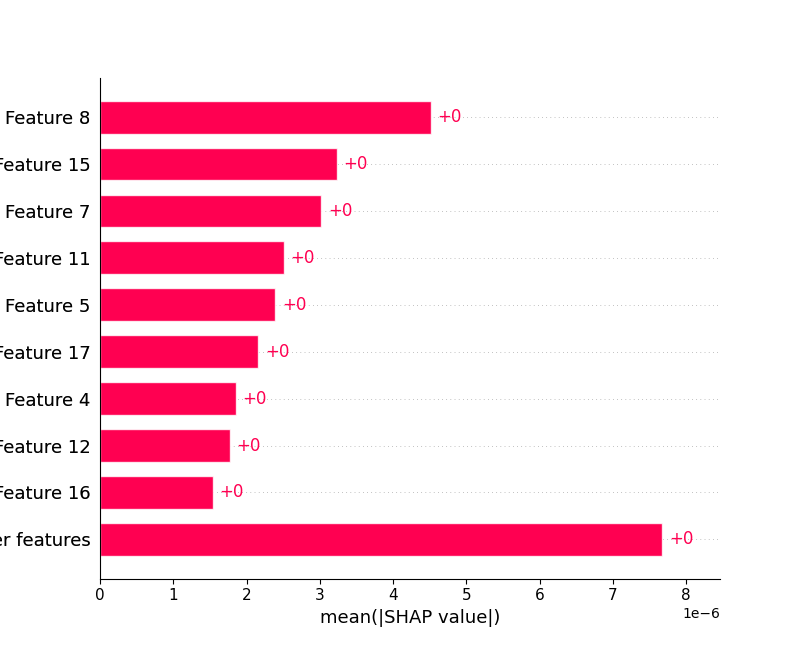
\includegraphics[width=0.6\textwidth]{case2_shap_values.png}
\end{figure}

\section{Modifications}
The structure and the training of the model can be modified by changing the values of \\ 

\noindent\rule{17cm}{0.4pt}\\
experiment\_settings = dict(location\_id=116.0, value\_type\_id=11, activation='sigmoid', layers\_number=4, neurons\_number=[32, 16, 8, 4, 4], loss='mean\_squared\_error', optimizer\_name='SGD', epochs=200,                     batch\_size=32, window\_size=pt1.window\_size, split\_percentage=pt1.split\_percentage)
\noindent\rule{17cm}{0.4pt}\\

and then running function\\

\noindent\rule{17cm}{0.4pt}\\
build\_and\_evaluate\_model\_target\_data()\\
\noindent\rule{17cm}{0.4pt}\\

in main.py.


%\pagebreak
%\bibliographystyle{apalike}
%\bibliography{srt}

\end{document}
